\documentclass[12pt]{article}
\usepackage{url,amsmath,setspace,amssymb}
\usepackage{listings}
\usepackage{caption}
\usepackage{tcolorbox}
\usepackage{tikz}
\usepackage{xcolor}
\usepackage{color}
\usepackage{cite}
\usepackage{graphicx}
\usepackage{xassoccnt}
\usepackage{algorithm}
\usepackage{algpseudocode}
\usepackage{booktabs}

\NewTotalDocumentCounter{totalpages}
\DeclareAssociatedCounters{page}{totalpages}

%**********************************************
%* Leave the page configuration as is
\setlength{\oddsidemargin}{.25in}
\setlength{\evensidemargin}{.25in}
\setlength{\textwidth}{6.25in}
\setlength{\topmargin}{-0.4in}
\setlength{\textheight}{8.5in}

\renewcommand{\thepage}{9-\arabic{page}}
\newcommand{\heading}[5]{
    \noindent
    \begin{center}
        \framebox[\textwidth]{
            \begin{minipage}{0.9\textwidth}
                \onehalfspacing
                {\textbf {#1}}

                {\centering \Large #5

                }\medskip
                {#3 \hfill #2 \hfill #4}
            \end{minipage}
        }
    \end{center}
}

\lstnewenvironment{myalgorithm}[1][]
{
    \lstset{
        mathescape=true,
        frame=none,
        numbers=none,
        basicstyle=\normalsize,
        keywordstyle=\color{black}\bfseries\em,
        keywords={,input, output, return, datatype, function, in, if, else, foreach, while, begin, end, },
        numbers=left,
        xleftmargin=.04\textwidth,
        #1
    }
}
{}

\newtcolorbox{alert}[1]{
    colback=red!5!white, colframe=red!75!white,fonttitle=\bfseries, title = #1}

\newtcolorbox{commentbox}[1]{
    colback=black!5!white, colframe=black!75!white,fonttitle=\bfseries, title = #1}

\newcommand{\handout}[5]{\heading{#1}{#2}{#3}{#4}{#5}}

\begin{document}

    \handout{650.060 - Small Project in Artificial Intelligence and Cybersecurity}{Summer Term 2022/2023}{Francesco Bombassei De Bona}{12138677}{An API for Mutual Information estimation}


    \section{Introduction}\label{sec:intro}
    Mutual Information (MI) plays a pivotal role in the realms of artificial intelligence and cybersecurity.
    It serves as a measure to quantify the amount of information shared between two variables.
    In the domain of cybersecurity, especially in side-channel attacks, an accurate estimation of MI can be the difference between a successful breach and a failed attempt.
    However, the current methodologies for estimating MI, especially in mixed cases, present challenges in terms of accuracy and computational efficiency.
    This project aims to address these challenges by introducing a publicly available C++ API that employs the methodologies presented in~\cite{chowdhury_leakage_2022}.
    Furthermore, we provide a comparative analysis of our proposed implementation with the traditional histogram estimator method.

    \section{Background and terminology}\label{sec:background}

    \subsection{Mutual Information}\label{subsec:mi}
    Mutual Information (MI) is a measure of the statistical dependence between two random variables.
    In the context of side-channel analysis, MI is used to quantify the dependence between an observed leakage and a secret key.
    Higher values of MI indicate a stronger dependence between the two variables.
    Thus, an higher MI value leads to a higher leakage of information about the secret key by observing a side-channel trace.

    The MI between two random variables $X$ and $Y$ is defined as:
    \begin{align}
        I(X;Y) &= H(X) - H(X|Y) \\ &= H(X) + H(Y) - H(X,Y)\label{eq:mi}
    \end{align}
    where $H(X)$ is the entropy of $X$, $H(X|Y)$ is the conditional entropy of $X$ given $Y$ and is defined as \[H(X|Y) = \begin{cases}
                                                                                                                              \sum_y p(y) H(X|Y=y) & \text{if } Y \text{ is discrete} \\ \int_y p(y) H(X|Y=y) dy & \text{if } Y \text{ is continuous}
    \end{cases}\] and $H(X,Y)$ is the joint entropy of $X$ and $Y$.

    As presented in~\cite{chowdhury_leakage_2022}, it's possible to observe three different cases of MI:
    \begin{itemize}
        \item $X$ and $Y$ discrete that leads to the discrete MI;
        \item $X$ and $Y$ continuous that leads to the continuous MI;
        \item $X$ discrete and $Y$ continuous that leads to the mixed MI\@.
    \end{itemize}

    In this work, we focus on the mixed MI case.

    For this case there are two different ways to compute the MI between $X$ and $Y$: using an estimator for the conditional/joint density in combination with the H2 or H3 formulas; or using an estimator based on nearest neighbors search.

    Side-channel analysis is a technique where attackers try to find a correlation between information leaked from physical implementations of cryptographic algorithms (like power consumption or electromagnetic emissions) and the secret key used during the cryptographic operations.
    MI, in this context, quantifies the amount of information about the secret key that can be inferred from these leakages.

    The three different cases of MI—discrete-discrete, continuous-continuous, and discrete-continuous—have their unique applications.
    For instance, discrete-discrete MI might be used in analyzing categorical data, while continuous-continuous could be applied in regression analysis.
    The mixed MI, which is the focus of our work, is particularly challenging due to the inherent complexities in handling both discrete and continuous data types.

    \subsection{Histogram estimator}\label{subsec:hist}
    The histogram estimator is a method for estimating the MI between two random variables $X$ and $Y$.
    The core idea behind the histogram estimator is to discretize the continuous random variables into bins and then compute the mutual information based on the joint and marginal frequencies of these bins.
    The MI between $X$ and $Y$ is then estimated using the H2 equation as:
    \begin{equation}
        I(X;Y) = H(Y) - H(Y|X)\label{eq:hist}
    \end{equation}
    where $H(Y)$ is the entropy of $Y$ and $H(Y|X)$ is the conditional entropy of $Y$ given $X$.

    \subsection{GKOV estimator}\label{subsec:gkov}
    The GKOV estimator is a method for estimating the MI between two random variables $X$ and $Y$ introduced by Gao, Krishnan, Oh and Vishwanath ~\cite{gao_estimating_2017}.
    This estimator can be used on a combination of discrete and continuous random variables.
    The GKOV estimator is defined as:
    \begin{equation}
        I_n(X;Y) = \frac{1}{n} \sum_{i=1}^n \hat{I}_i = \sum_{i=1}^n \left( \psi(\tilde{t}_i) + \log n - \log(n_{x,i}+1) - \log(n_{y,i}+1) \right)\label{eq:gkov}
    \end{equation}
    where $\psi$ is the digamma function.


    \section{Project Execution}\label{sec:execution}
    The project aimed to develop a C++ API for the GKOV estimator, the histogram estimator, and a simulator for the leakage of a device.
    All the code was written in C++ and using an OO approach.

    In the `Simulator` subsection, our chosen leakage model is reflective of many real-world scenarios where a device's physical leakages (like power consumption) can be modeled as a function of its cryptographic operations, added with some noise.
    This noise can arise from various sources, including environmental factors or inherent device fluctuations.

    \subsection{GKOV estimator}\label{subsec:gkov_impl}
    The GKOV estimator was implemented as described in~\cite{gao_estimating_2017}.
    The implementation is based on the class \texttt{GKOVEstimator} which is initialized with the callback function to compute the value $t_n$ as described in~\cite{chowdhury_leakage_2022}.
    The class \texttt{GKOVEstimator} provides the method \texttt{estimate} which takes as input the discrete variable $X$, the continuous variable $Y$, and the dimension of the two variables.
    The method \texttt{estimate} returns the estimated MI between $X$ and $Y$.
    Under the hood, the method \texttt{estimate} computes the value $t$, builds the matrix data starting from the discrete and continuous variables, builds the search trees for the two single variables and the combined matrix, and finally computes the GKOV estimator as described in~\cite{chowdhury_leakage_2022}.

    To perform the nearest neighbors search, the project makes usage of the MLPack library~\cite{mlpack2023}.
    The class \texttt{GKOVEstimator} makes usage of the class \texttt{mlpack::neighbor::NeighborSearch} to perform the nearest neighbors search over the combined matrix built from the discrete and continuous variables.
    While to perform the computation of lines 4, 8, and 9 of Algorithm 1 in~\cite{chowdhury_leakage_2022}, the class \texttt{GKOVEstimator} makes usage of the class \texttt{mlpack::neighbor::RangeSearch} to perform the distance search over the combined variables and the single variables.
    In particular, the tree used for both types of search is the \texttt{mlpack::tree::BallTree}.

    \subsection{Histogram estimator}\label{subsec:hist_impl}
    The histogram estimator was implemented to be used as a baseline for comparing the GKOV estimator.
    Following the description in Section~\ref{subsec:hist}, the histogram estimator was implemented as a class \texttt{HistogramEstimator}.
    The class \texttt{HistogramEstimator} is initialized with the number of dimensions of the continuous variable $Y$, the number of bins for each dimension, and the ranges of the bins.
    The underlying assumption about the ranges is that the bins are equally spaced.
    The class \texttt{HistogramEstimator} provides the method \texttt{estimate} which takes as input the discrete variable $X$, its probability distribution, the continuous variable $Y$, the size of the two variables and the dimension of the $Y$ variable.

    The method \texttt{estimate} makes usage of the methods \texttt{build\_histogram}, \texttt{pdf\_entropy}, and \texttt{conditional\_entropy} to compute the MI between $X$ and $Y$.
    \texttt{build\_histogram} builds histogram of $Y$ based on the dimensions of the variable and computes the pdf of the histogram.
    To ensure the efficiency of the histogram estimator, the method makes usage of the GSL library~\cite{galassi_gnu_2009} for building the 1D and 2D histograms.
    The method \texttt{pdf\_entropy} computes the entropy of the pdf of $Y$.
    The method \texttt{conditional\_entropy} computes the conditional entropy of $Y$ given $X$.
    Finally, the method \texttt{estimate} returns the MI between $X$ and $Y$ computed as described in equation~\ref{eq:hist}.

    \subsection{Simulator}\label{subsec:sim}
    The simulator was implemented to provide a way to test the GKOV estimator and the histogram estimator.
    This class has the purpose of simulating the leakage of a device using the following model:
    \begin{equation}
        \text{leakage} = \text{leakage\_function}(\text{crypto\_function}(key, \text{plaintext})) + \text{noise}\label{eq:sim}
    \end{equation}
    where \texttt{leakage\_function} is the function that simulates the leakage of the device, \texttt{crypto\_function} is the function that simulates the cryptographic function of the device, and \texttt{noise} is the noise added to the leakage.
    At time of writing, the simulator supports gaussian and laplacian noise distributions but the code was made to be easily extensible to other distributions.
    Instead, the cryptographic function is passed as argument of the methods of the simulator.

    Regarding the type of trace that can be simulated, the simulator supports one dimensional traces, but new can be easily added by extending the main class.

    Finally, the simulator saves the simulated traces in a HDF5 file to allow the user to use the traces for further analysis.

    \subsection{Utilities}\label{subsec:utils}
    The project provides a class that implements some utilities used by the other classes in the project.

    In particular, the class \texttt{Utils} provides the methods:
    \begin{itemize}
        \item \texttt{flatten} and \texttt{to\_gkov\_format} to convert an n-dimensional array to, respectively, a 1-dimensional array and a 2-dimensional array;
        \item \texttt{compute\_distribution} to compute the distribution of a discrete variable;
        \item \texttt{read\_traces} and \texttt{write\_traces} to read and write traces from and to a HDF5 file.
    \end{itemize}


    \section{Project Evaluation}\label{sec:evaluation}
    The project was evaluated by comparing the GKOV estimator with the histogram estimator.

    \subsection{Simulation of the traces}\label{subsec:phase1}
    The first phase of the evaluation was to simulate the traces of a device.
    The \texttt{Simulator} class was used to achieve this goal.

    The simulation was done for an increasing length of the traces, from 10 to 163840 samples.
    The traces were simulated using the AES-128 algorithm with a random key, a gaussian noise with mean 0 and standard deviation 1, and a leakage function that computes the Hamming weight of the intermediate value of the AES-128 algorithm.
    The traces were saved in a HDF5 file to allow the user to use the traces for further analysis along with the secret key saved as attribute of the HDF5 file.

    \subsection{Setup of the experiments}\label{subsec:phase2}
    The second phase of the evaluation was to set up the experiments.
    From a first run of a potential attack, it was notice that the computation of the GKOV estimator was computationally expensive.
    To improve the performance of the GKOV estimator, the usage of the Python library \texttt{ray}~\cite{moritz2018ray} was considered.

    The idea was to use the Python library \texttt{ray} to parallelize the computation of the GKOV estimator across a cluster of machines.
    This library is focused on the parallelization of AI tasks, but it can be used for any kind of parallelization.

    The parallelization of the attack was done by generating a list of tasks, where each task is the computation of the MI between a single trace and one of the 256 possible values of the secret key.
    The list of task was then split across the machines of the cluster.
    This procedure was repeated for each trace generated in the previous phase.

    AWS was chosen as platform for the deployment of the cluster since it is natively supported by \texttt{ray}.
    The machines of the cluster were configured as follows:
    \begin{itemize}
        \item 1 head node of the type \texttt{c6a.xlarge} with 4 vCPUs and 8 GB of RAM, responsible for the coordination of the cluster and saving the results of the computation;
        \item 30 worker nodes of the type \texttt{c6a.large} with 2 vCPUs and 4 GB of RAM, responsible for the computation of MI values using both the GKOV estimator and the histogram estimator.
    \end{itemize}
    All the vCPUs of the machines are based on 3rd generation AMD EPYC processors with a turbo clock speed of 3.6 GHz.

    \subsection{Attack}\label{subsec:phase3}
    The third phase of the evaluation was to run the attack.

    \begin{algorithm}
        \caption{Attack}\label{alg:attack}
        \begin{algorithmic}[1]
            \Require{Filename, Key}
            \Ensure{Estimated MI values}
            \State $traces \gets \text{read\_traces}(Filename)$

            \State $Y\_gkov \gets \text{to\_gkov\_format}(traces)$ \Comment{Convert traces to GKOV format}
            \State $Y\_hist \gets \text{flatten}(traces)$ \Comment{Convert traces to histogram format}

            \State $gkov\_estimator \gets \text{GKOVEstimator}(t)$
            \State $hist\_estimator \gets \text{HistogramEstimator}(dims, bins, range)$

            \State $X \gets \text{hamming\_weight}(\text{aes\_intermidiate}(traces, Key))$ \Comment{Compute the discrete variable}

            \State $gkov\_estimates \gets gkov\_estimator.estimate(X, Y\_gkov, sizeOfX, sizeOfY)$ \Comment{Compute the GKOV estimates}
            \State $hist\_estimates \gets hist\_estimator.estimate(X, pX, Y\_hist, size, dims)$ \Comment{Compute the histogram estimates}
        \end{algorithmic}
    \end{algorithm}

    The attack was implemented as described in Algorithm~\ref{alg:attack} with the following parameters:

    \begin{itemize}
        \item \texttt{t} was set to be $\log_{10}$
        \item \texttt{dims} was set to 1;
        \item \texttt{bins} was set to 10;
        \item \texttt{range} was set to $[\min Y, \max Y]$;
        \item \texttt{pX} was set to the distribution of 1s in the intermediate value of the AES-128 algorithm;
    \end{itemize}

    \subsection{Results}\label{subsec:results}
    After running the attack, the results were collected from the cluster and analyzed.
    The results were collected in a JSON file using the following format:
    \begin{lstlisting}[label={lst:lstlisting}]
    {
        key : {
            "gkov": value,
            "hist": value
        }
    }
    \end{lstlisting}

    The results are presented in the following table:

    \vspace{0.5cm}
    \begin{tabular}{rllrll}
        \toprule
        samples & key & gkov & gkov\_mi  & hist & hist\_mi      \\
        \midrule
        10      & 235 & 20   & -1.426090 & 32   & 2.05532       \\
        20      & 233 & 244  & -1.225250 & 176  & 1.58543       \\
        40      & 17  & 104  & -1.084880 & 167  & 0.518031      \\
        80      & 140 & 140  & 0.086083  & 86   & -3.3962       \\
        160     & 115 & 115  & 0.220301  & 97   & -9.97996      \\
        320     & 55  & 55   & 0.177586  & 55   & -22.8171      \\
        640     & 107 & 107  & 0.246235  & 107  & -50.9727      \\
        1280    & 131 & 131  & 0.369563  & 222  & -99.1721      \\
        2560    & 252 & 252  & 0.368122  & 252  & -229.192      \\
        5120    & 12  & 12   & 0.365723  & 12   & -450.422      \\
        10240   & 238 & 238  & 0.422796  & 238  & -900.454      \\
        20480   & 186 & 186  & 0.404086  & 186  & -1847.61      \\
        40960   & 120 & 120  & 0.412238  & 168  & -3492.770000  \\
        81920   & 114 & 114  & 0.407635  & 15   & -7112.370000  \\
        163840  & 179 & 179  & 0.440852  & 206  & -14527.300000 \\
        \bottomrule
    \end{tabular}
    \vspace{0.5cm}

    First, it can be observed that the GKOV estimator is more accurate than the histogram estimator.
    In fact, the GKOV estimator is able to recover the correct key for all the traces if the number of samples is greater than 80, while the histogram estimator is able to recover the correct key only for 6 traces over the 15 traces.
    It is unclear why the histogram estimator is not able to recover the correct key for all the traces, but it is possible that the parameters of the histogram estimator were not chosen correctly.
    In fact, the choice of the correct binning size is not trivial and it is possible that the binning size chosen for the histogram estimator is not the correct one.

    Second, it can be observed, by plotting the MI values of the GKOV estimator, that these values seem to converge to a value between 0.4 and 0.5, as shown in Figure~\ref{fig:gkov_mi}.
    This is in line with the results presented in~\cite{chowdhury_leakage_2022} where it is shown that the GKOV estimator converge to the true MI value as the number of samples increases.

    \begin{figure}[H]
        \centering
        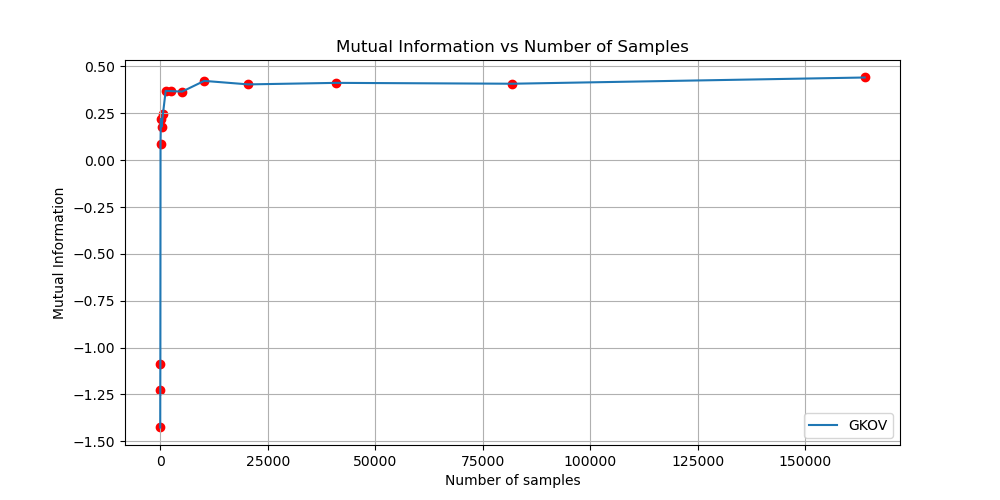
\includegraphics[width=0.8\textwidth]{../data/plots/gkov_mi}
        \caption{GKOV MI values}
        \label{fig:gkov_mi}
    \end{figure}

    \begin{figure}[H]
        \centering
        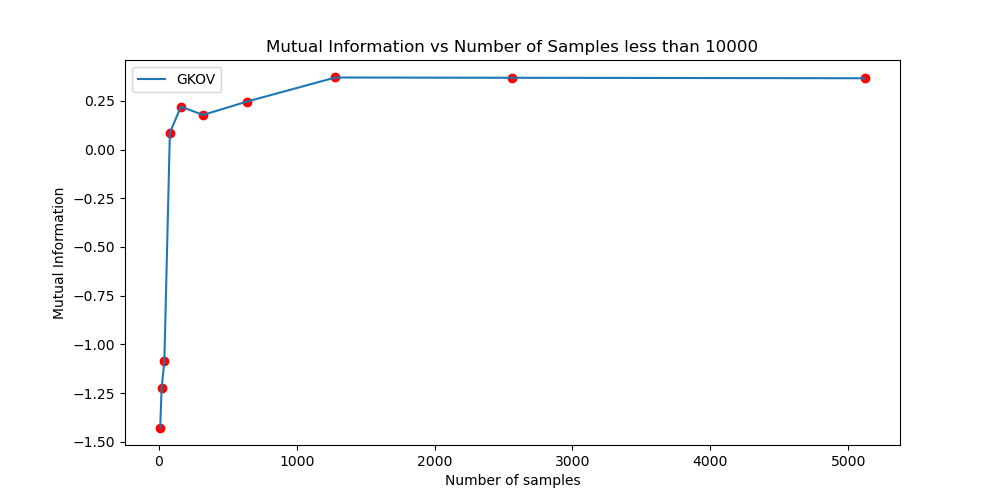
\includegraphics[width=0.8\textwidth]{../data/plots/gkov_mi_10000}
        \caption{GKOV MI values for less than 10000 samples}
        \label{fig:gkov_mi_10000}
    \end{figure}

    \section{Conclusion}
    Our project successfully introduces a C++ API for estimating Mutual Information, with a particular focus on the mixed MI case.
    The GKOV estimator, as demonstrated, offers a more accurate and reliable estimation compared to the traditional histogram estimator.
    This advancement holds significant implications for the field of cybersecurity, especially in the realm of side-channel attacks.
    Future work could delve into optimizing the histogram estimator's parameters or exploring other estimation methodologies to further enhance accuracy and computational efficiency.

    \newpage
    \bibliography{references}
    \bibliographystyle{acm}
\end{document}



